\chapter*{Experiment 5 - clap4Led}
\addcontentsline{toc}{chapter}{Experiment 5 - clap4Led}
We wire up the experiment as shown in the diagram fig:~\ref{fig:exp5_microphone}. And upload the sketch code in the next section on page:~\pageref{sketch:exp5}.

%
\begin{figure}[ht]
	\centering
	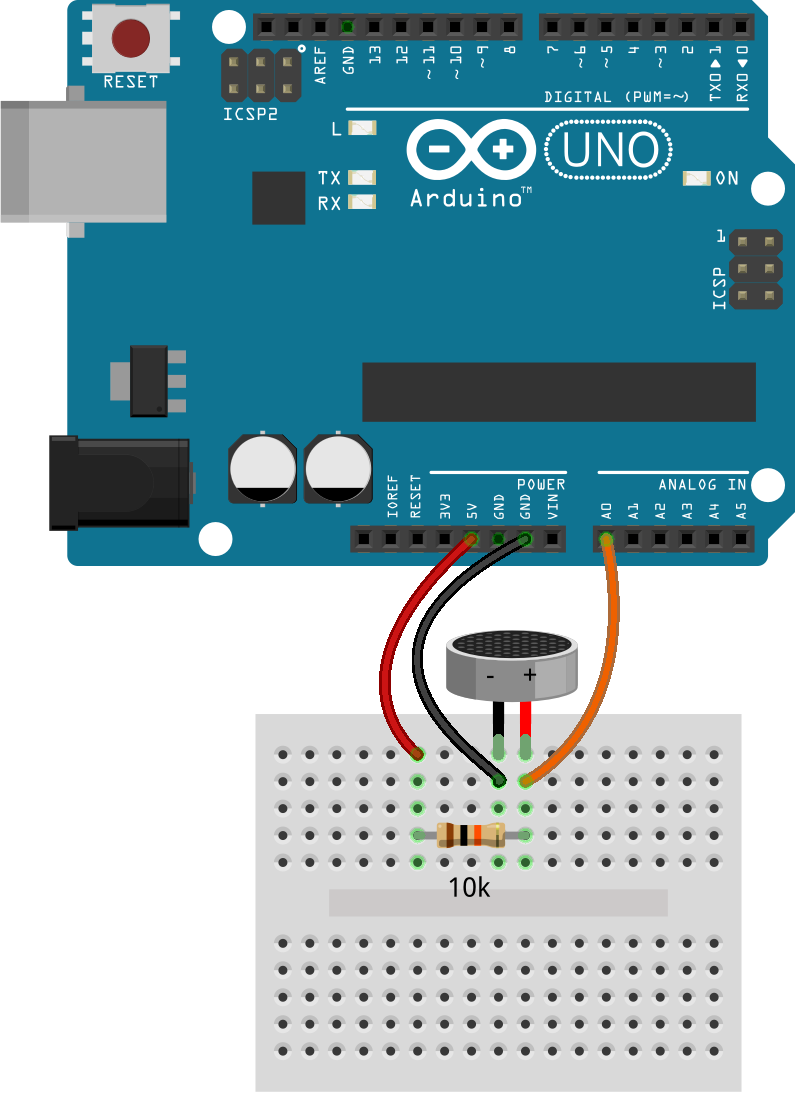
\includegraphics[width=8cm]{images/21}
	\caption{Microphone Activated Circuit}
	\label{fig:exp5_microphone}
\end{figure}
%

The microphone module is polarised, which means it has a positive and negative terminal which must be correctly placed in the circuit in order to function as expected. Please examine the diagram fig:~\ref{fig:exp5_microphone_polarity} on page:~\pageref{fig:exp5_microphone_polarity} to correctly identify which leg is positive and which is negative.

When this circuit is complete, the LED onboard the Arduino will flash when the microphone detects sound.

%
\begin{figure}[ht]
	\centering
	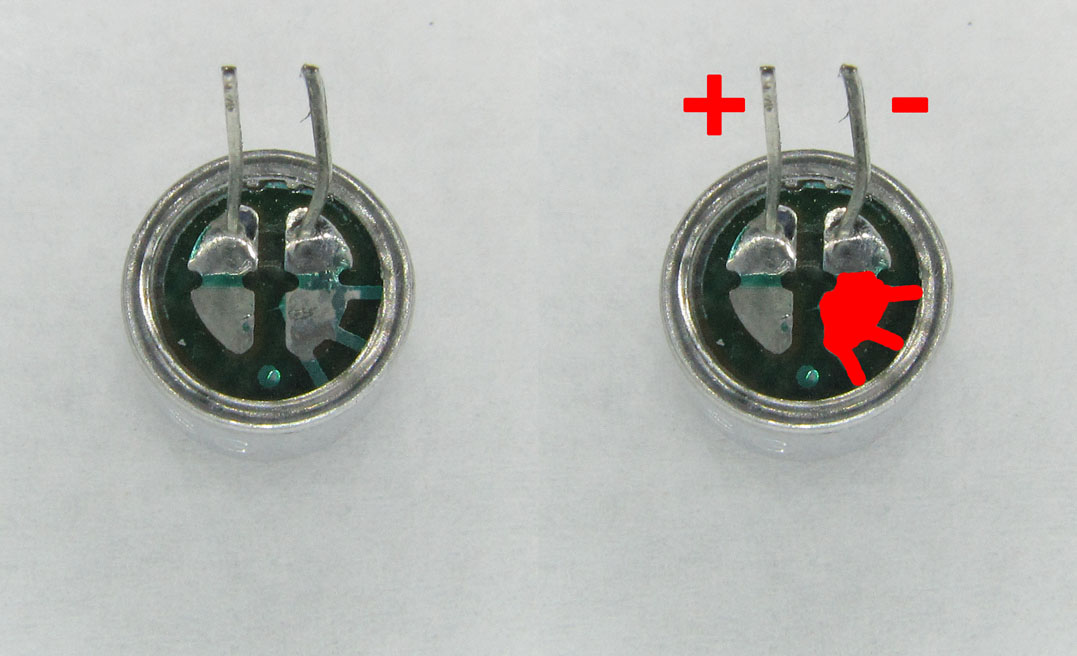
\includegraphics[width=12cm]{images/22}
	\caption{Microphone Module Polarity}
	\label{fig:exp5_microphone_polarity}
\end{figure}
%


\newpage
\section*{Sketch Code}
\label{sketch:exp5}
\begin{lstlisting}
/*
<<<<<<< HEAD
Sample code to work with a Thermistor

Author: Anton Krug
Licence: Apache 2.0
*/

//global variables
int readValue;
int maximumValue;
int minimumValue; 


// will reset maximum and minimum values only when we call it
void resetMaximumAndMinimum() 
{
  maximumValue = 0;             // set maximum to lowest value possible
  minimumValue = 32767;         // set minimum to highest value possible
}


// this runs only once on the startup
void setup() 
{
  // initialize built-in LED light at digital pin 13 as an output
  pinMode(13, OUTPUT);           
  resetMaximumAndMinimum();
}


// the loop runs over and over again forever
void loop() 
{
  // read current value from the microphone
  readValue = analogRead(A0);     

  // if read value is smaller than minimum then set it as the new minimum
  if (readValue < minimumValue)   
  {
    minimumValue = readValue;     
  }

  // if read value is bigger than maximum then set it as the new maximum
  if (readValue > maximumValue)   
  {
    maximumValue = readValue;     
  }

  // Change the 10 constant to adjust the sensitivity.
  //   To 20 if you want the light triggered on louder claps   
  //   Ti 5  if you want the light triggered on quieter noises 
  //   Feel free to experiment with the values.
  if ( (maximumValue - minimumValue) > 10 ) 
  {
    digitalWrite(13, HIGH);       // turn the LED on (HIGH is the voltage level)
    delay(2 * 1000);              // wait for 2 seconds (2 * 1000ms)
    digitalWrite(13, LOW );       // turn the LED off by making the voltage LOW

    // if we wouldn't clear the max & min then after first trigger it would get 
    // triggered every single time no matter what read values were
    resetMaximumAndMinimum();     
  }
}

=======
Phenakistoscope
Turns on an LED on then off 20 times a second in order to activate the Phenakistoscope
*/

// the setup function runs once when you press reset or power the board
void setup() {
  // initialize digital pin 13 as an output.
  pinMode(13, OUTPUT);
}

// the loop function runs over and over again forever
void loop() {
  // turn the LED on 
  // (HIGH is the voltage level)
  digitalWrite(13, HIGH);
	
  //wait for 10 milliseconds
  delay(10);
	
  // turn the LED off by making 
  // the voltage LOW
  digitalWrite(13, LOW);    
	            
  // wait for 30 milliseconds              
  delay(30);
}
>>>>>>> 0581ff186ec5408b185455777b58f0f20d96f775
\end{lstlisting}